% -*- mode: latex; mode: flyspell; ispell-local-dictionary: "en_US"; coding: utf-8 -*-

\documentclass{standalone}
\usepackage{graphicx}
\usepackage{tikz}
\usepackage{pgfplots}
\usepgfplotslibrary{groupplots}
\pgfplotsset{compat=newest}
\begin{document}

% IMPORT-DATA result result.txt

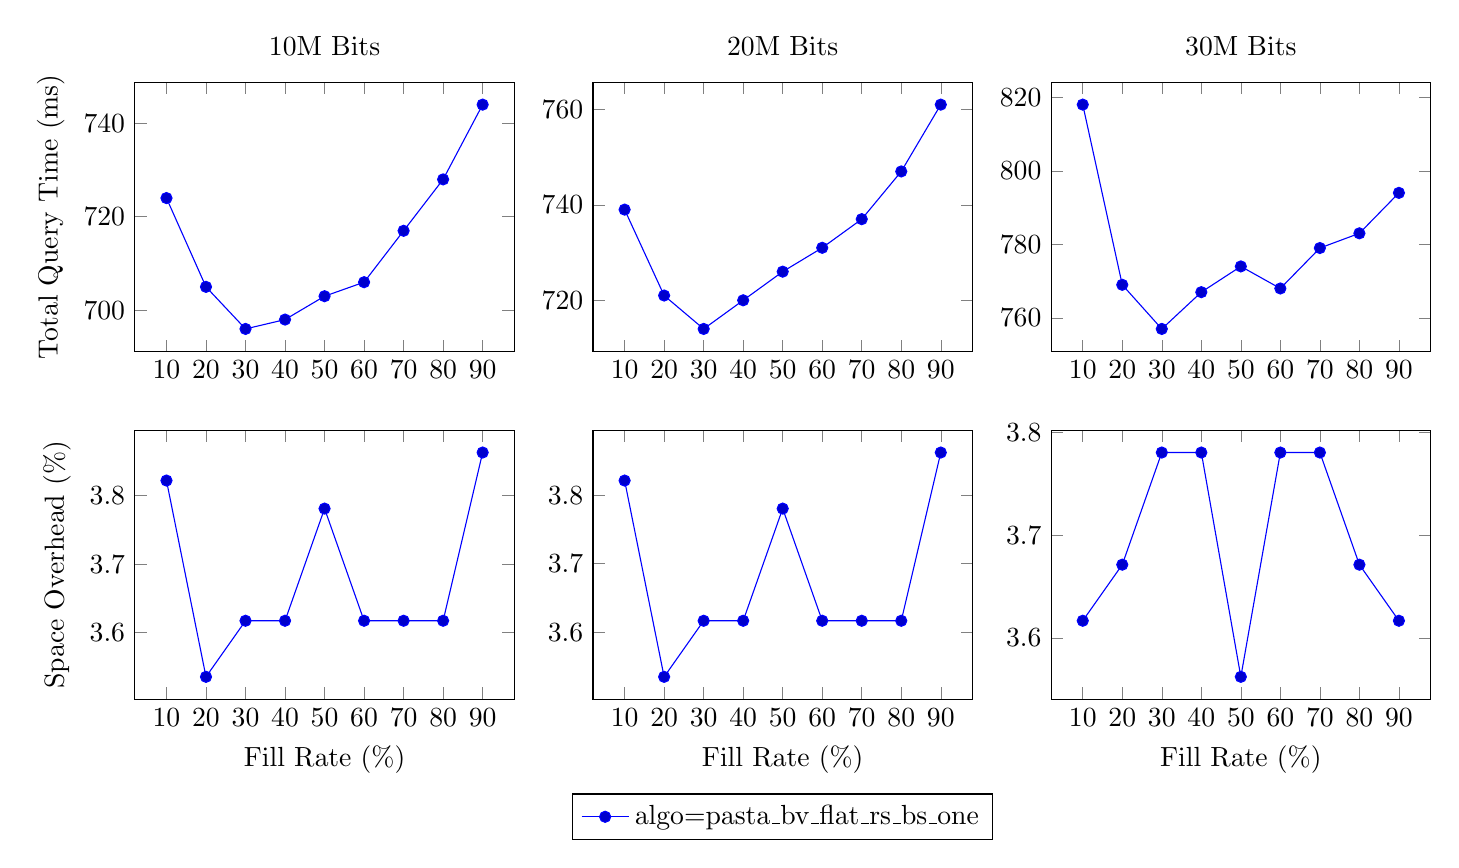
\begin{tikzpicture}
    \begin{groupplot}[group style={group size= 3 by 2},height=5cm,width=6.4cm]

    \nextgroupplot[title={10M Bits},ylabel={Total Query Time (ms)},xtick=data]
%% MULTIPLOT(algo) SELECT fill_percentage AS x, total_select_query_time AS y, MULTIPLOT
%% FROM result WHERE bit_size=10000000 AND correctness_check = 'pass' GROUP BY MULTIPLOT,x ORDER BY MULTIPLOT,x
\addplot coordinates { (10,724) (20,705) (30,696) (40,698) (50,703) (60,706) (70,717) (80,728) (90,744) };
\addlegendentry{algo=pasta\_bv\_flat\_rs\_bs\_one};
\legend{};

    \nextgroupplot[title={20M Bits},xtick=data]
%% MULTIPLOT(algo) SELECT fill_percentage AS x, total_select_query_time AS y, MULTIPLOT
%% FROM result WHERE bit_size=20000000 AND correctness_check = 'pass' GROUP BY MULTIPLOT,x ORDER BY MULTIPLOT,x
\addplot coordinates { (10,739) (20,721) (30,714) (40,720) (50,726) (60,731) (70,737) (80,747) (90,761) };
\addlegendentry{algo=pasta\_bv\_flat\_rs\_bs\_one};
\legend{};

    \nextgroupplot[title={30M Bits},,xtick=data]
%% MULTIPLOT(algo) SELECT fill_percentage AS x, total_select_query_time AS y, MULTIPLOT
%% FROM result WHERE bit_size=30000000 AND correctness_check = 'pass' GROUP BY MULTIPLOT,x ORDER BY MULTIPLOT,x
\addplot coordinates { (10,818) (20,769) (30,757) (40,767) (50,774) (60,768) (70,779) (80,783) (90,794) };
\addlegendentry{algo=pasta\_bv\_flat\_rs\_bs\_one};
\legend{};

    \nextgroupplot[xlabel={Fill Rate (\%)},ylabel={Space Overhead (\%)},xtick=data]
%% MULTIPLOT(algo) SELECT fill_percentage AS x, 100.0 / bit_size * (rs_construction_mem * 8) AS y, MULTIPLOT
%% FROM result WHERE bit_size=10000000 AND correctness_check = 'pass' GROUP BY MULTIPLOT,x ORDER BY MULTIPLOT,x
\addplot coordinates { (10,3.82208) (20,3.53536) (30,3.61728) (40,3.61728) (50,3.78112) (60,3.61728) (70,3.61728) (80,3.61728) (90,3.86304) };
\addlegendentry{algo=pasta\_bv\_flat\_rs\_bs\_one};
\legend{};

    \nextgroupplot[xlabel={Fill Rate (\%)},xtick=data,legend style={at={(0.5,-0.35)},anchor=north}]
%% MULTIPLOT(algo) SELECT fill_percentage AS x, 100.0 / bit_size * (rs_construction_mem * 8) AS y, MULTIPLOT
%% FROM result WHERE bit_size=20000000 AND correctness_check = 'pass' GROUP BY MULTIPLOT,x ORDER BY MULTIPLOT,x
\addplot coordinates { (10,3.82144) (20,3.53472) (30,3.61664) (40,3.61664) (50,3.78048) (60,3.61664) (70,3.61664) (80,3.61664) (90,3.8624) };
\addlegendentry{algo=pasta\_bv\_flat\_rs\_bs\_one};

    \nextgroupplot[xlabel={Fill Rate (\%)},xtick=data]
%% MULTIPLOT(algo) SELECT fill_percentage AS x, 100.0 / bit_size * (rs_construction_mem * 8)  AS y, MULTIPLOT
%% FROM result WHERE bit_size=30000000 AND correctness_check = 'pass' GROUP BY MULTIPLOT,x ORDER BY MULTIPLOT,x
\addplot coordinates { (10,3.61685) (20,3.67147) (30,3.78069) (40,3.78069) (50,3.56224) (60,3.78069) (70,3.78069) (80,3.67147) (90,3.61685) };
\addlegendentry{algo=pasta\_bv\_flat\_rs\_bs\_one};
\legend{};y

\end{groupplot}
\end{tikzpicture}
\end{document}
